\chapter{Model Hammersteina}
W przypadku modelu Hammersteina istota polega na rozdzieleniu dynamiki i statyki w sposób przedstawiony na rys. \ref{hamm_model}.

\begin{figure}[h!]
\centering
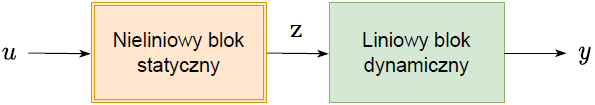
\includegraphics[width=\textwidth]{pictures/hamm_model}
\caption{Reprezentacja graficzna modelu Hammersteina.}
\label{hamm_model}
\end{figure}

\noindent Zatem sygnał sterujący trafia na blok nieliniowej statyki, gdzie jest przekonwertowany na sygnał $z = f(u)$, który następnie trafia na liniowy bloczek dynamiczny. 

\section{Nieliniowy blok statyczny}
Nieliniowość w charakterystyce statycznej została wprowadzono za pomocą logiki rozmytej (ang. \textit{fuzzy logic}), a konkretnie za pomocą modeli rozmytych Takagi-Sugeno. Zastosowano dwa podejścia, jedno standardowe z następnikami liniowymi, natomiast drugie z następnikami hiperbolicznymi.

\section{Następniki liniowe}
Zaczęto od rozmycia zmiennej wejściowej. Symulacyjnie wyznaczono odpowiednią liczbę zbiorów - w tym przypadku pięć.

\begin{figure}[h!]
\centering
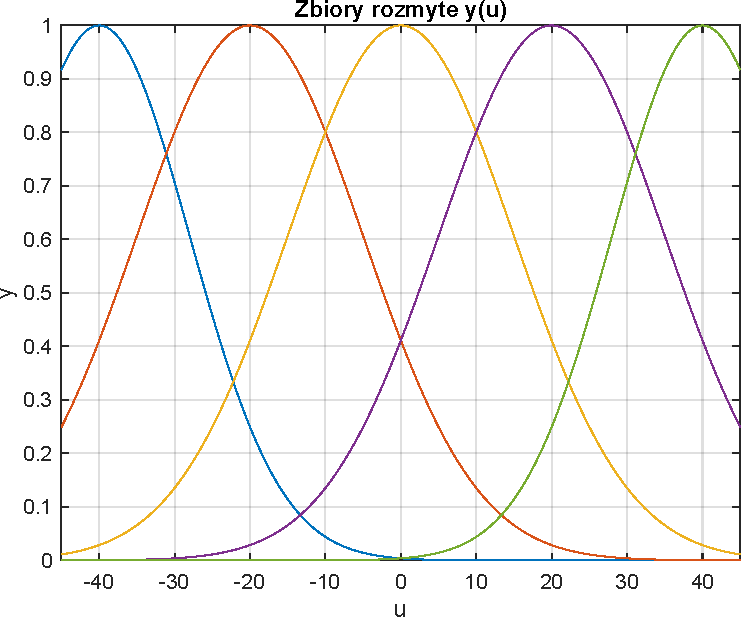
\includegraphics[width=0.5\textwidth]{pictures/fuzzy_set_ham}
\caption{Zbiory rozmyte - następniki liniowe.}
\label{hamm_model}
\end{figure}

\noindent Zastosowano następniki liniowe postaci:
\begin{equation}
\begin{aligned}
\text{Reguła 1: Jeśli} \quad u^1(k) \quad \text{jest} \quad &U_1, \quad \text{to}: \quad y^1(k) = a_1 + b_1 u^1(k) \\
\text{Reguła 2: Jeśli} \quad u^2(k) \quad \text{jest} \quad &U_2, \quad \text{to}: \quad y^2(k) = a_2 + b_2 u^2(k) \\ 
&\vdots \\
\text{Reguła 5: Jeśli} \quad u^5(k) \quad \text{jest} \quad &U_5, \quad \text{to}: \quad y^2(k) = a_5 + b_5 u^5(k) \\
\end{aligned}
\label{nastepniki_lin}
\end{equation}

Współczynniki w pierwszej iteracji dobierane były poprzez rozwiązanie nieliniowego zadania optymalizacji. W tym celu skorzystano z dostępnych funkcji programu MATLAB, tj. \verb+fminsearch()+, gdzie minimalizowaną funkcją był kwadrat różnicy wyjść wyznaczonej analitycznie charakterystyki statycznej i wyznaczanej charakterystyki rozmytej. Dane statyczne podzielono na zbiory uczący i weryfikujący z tą różnicą - w porównaniu do danych dynamicznych - że wzięto co drugą próbkę do każdego ze zbiorów. Dokładność aproksymacji charakterystyki statycznej przedstawiono na rys. \ref{static_hamm}, natomiast uzyskane błędy były na poziomie $\num{0.001}$. 

\begin{figure}[h!]
\centering
\subfloat[Zbiór uczący.]{
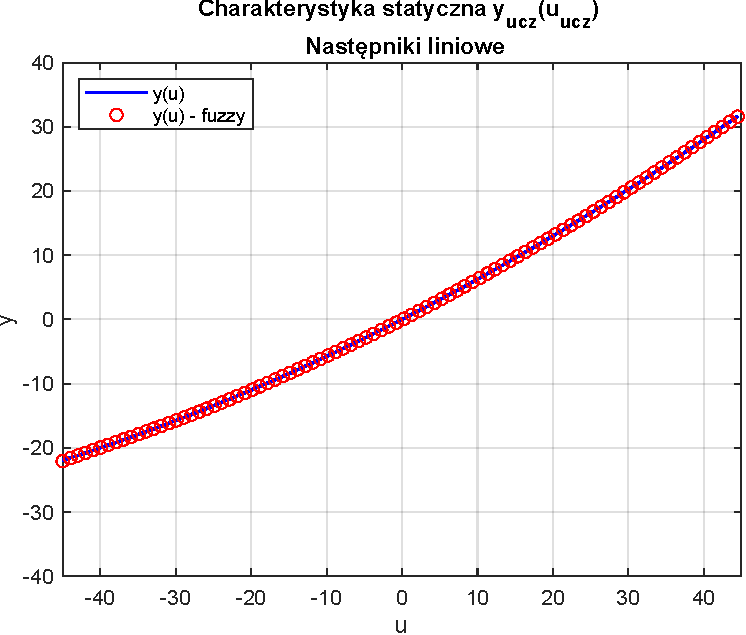
\includegraphics[width=0.45\textwidth]{pictures/static_char_ham_lin_ucz}}
\hfill
\subfloat[Zbiór weryfikujący]{
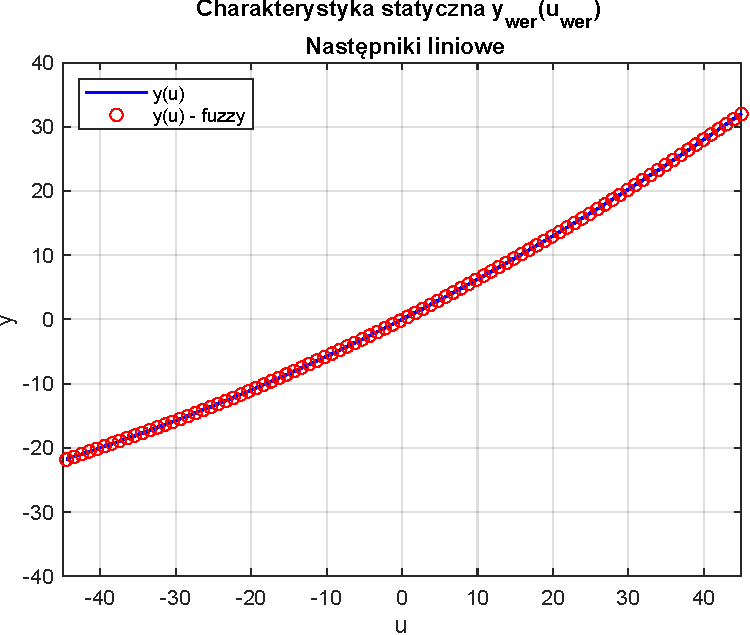
\includegraphics[width=0.45\textwidth]{pictures/static_char_ham_lin_wer}}
\caption{Aproksymacja charakterystyki statycznej przez model rozmyty - następniki liniowe.}
\label{static_hamm}
\end{figure}

Następnie korzystając z wcześniej opracowanego modelu dynamicznego wykonano szereg symulacji, sprawdzając jak zachowuje się układ w zależności od losowo wygenerowanych sygnałów sterujących. Efekty symulacji przedstawiono poniżej.

%%%%%%%%%%%%%%%%%%%%%% PIERWSZA SEKWENCJA %%%%%%%%%%%%%%%%%%%%%%

\begin{figure}[p!]

\begin{center}
\Large \textbf{I sekwencja} \\
\vspace{0.5cm}
\Large \textbf{Model dynamiczny}
\end{center}

\centering
\subfloat[Zbiór uczący.]{
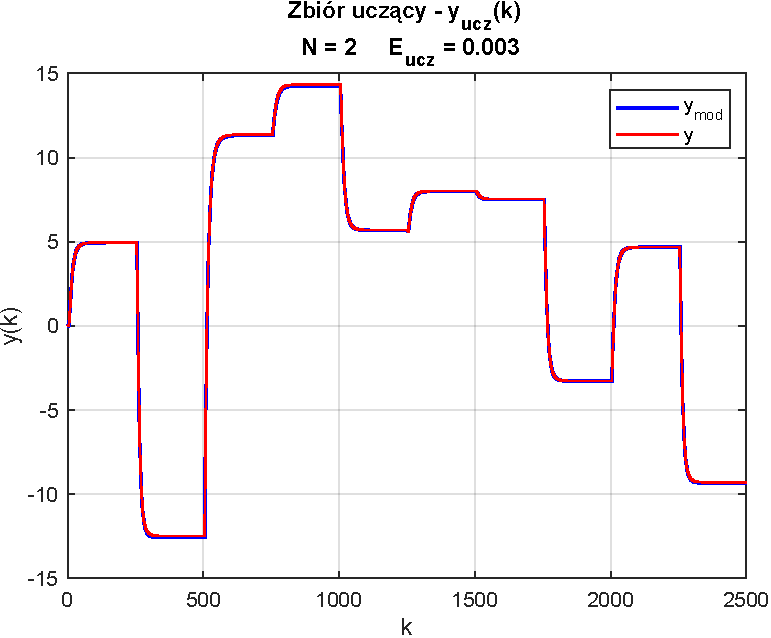
\includegraphics[width=0.45\textwidth]{pictures/arx_ucz_1}}
\hfill
\subfloat[Zbiór weryfikujący]{
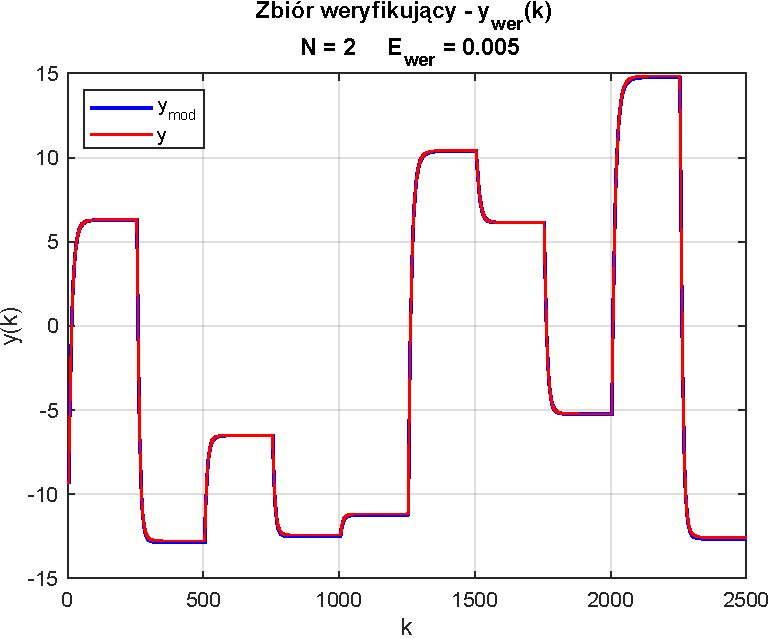
\includegraphics[width=0.45\textwidth]{pictures/arx_wer_1}}

\begin{center}
\Large \textbf{Model Hammersteina}
\end{center}

\subfloat[Zbiór uczący.]{
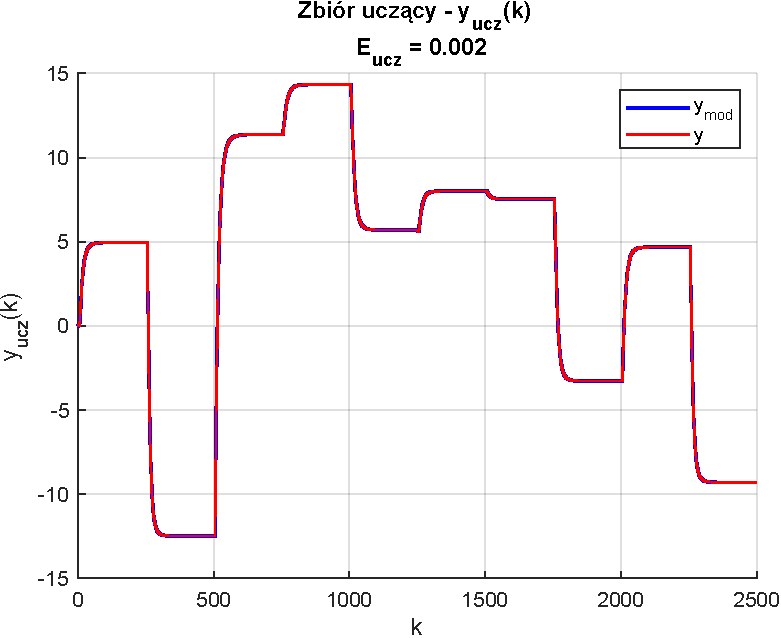
\includegraphics[width=0.45\textwidth]{pictures/arx_hamm_ucz_1}}
\hfill
\subfloat[Zbiór weryfikujący]{
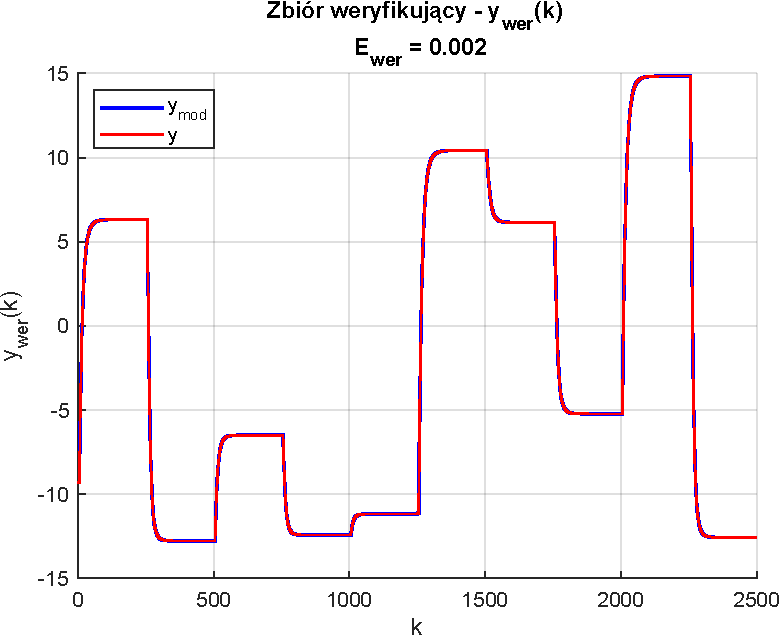
\includegraphics[width=0.45\textwidth]{pictures/arx_hamm_wer_1}}
\caption{Porównanie przebiegu sygnału wyjściowego modelu dynamicznego i modelu Hammesteina w trybie bez rekurencji.}
\end{figure}

\begin{figure}[p!]

\begin{center}
\Large \textbf{I sekwencja} \\
\vspace{0.5cm}
\Large \textbf{Model dynamiczny}
\end{center}

\centering
\subfloat[Zbiór uczący.]{
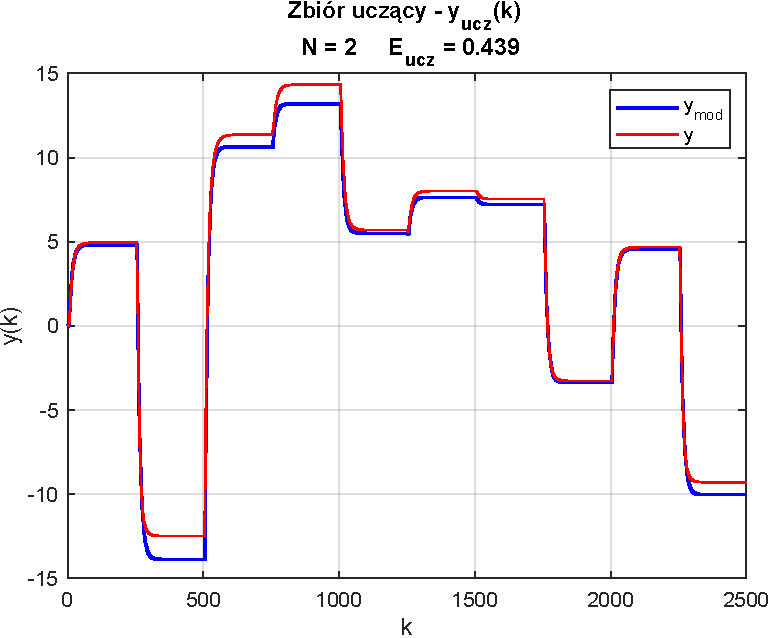
\includegraphics[width=0.45\textwidth]{pictures/oe_ucz_1}}
\hfill
\subfloat[Zbiór weryfikujący]{
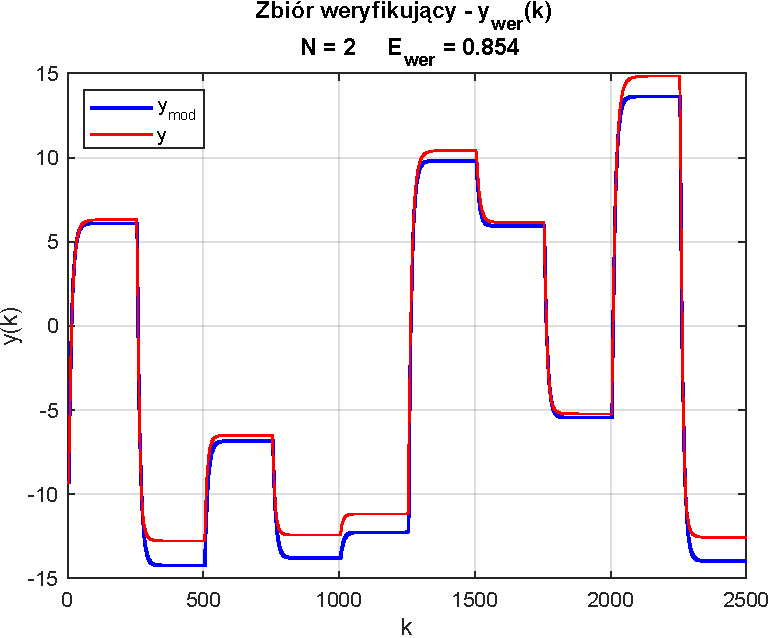
\includegraphics[width=0.45\textwidth]{pictures/oe_wer_1}}

\begin{center}
\Large \textbf{Model Hammersteina}
\end{center}

\subfloat[Zbiór uczący.]{
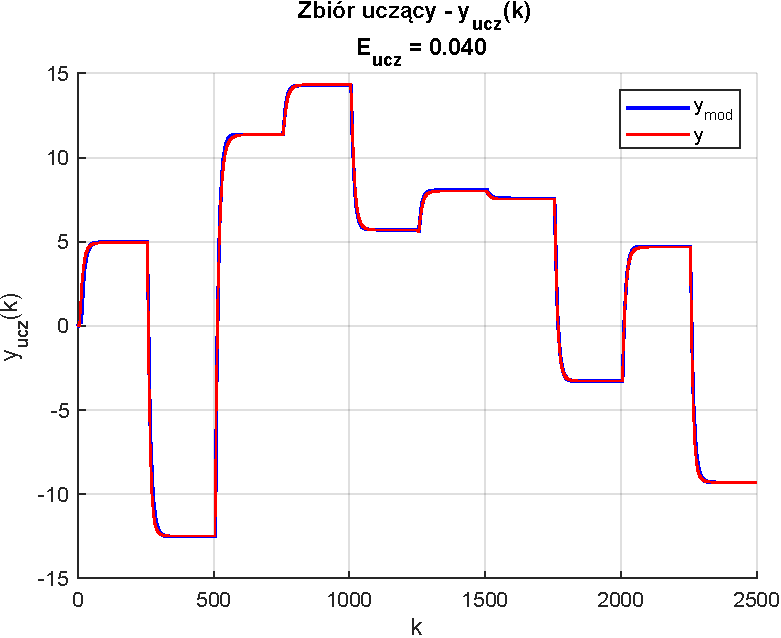
\includegraphics[width=0.45\textwidth]{pictures/oe_hamm_ucz_1}}
\hfill
\subfloat[Zbiór weryfikujący]{
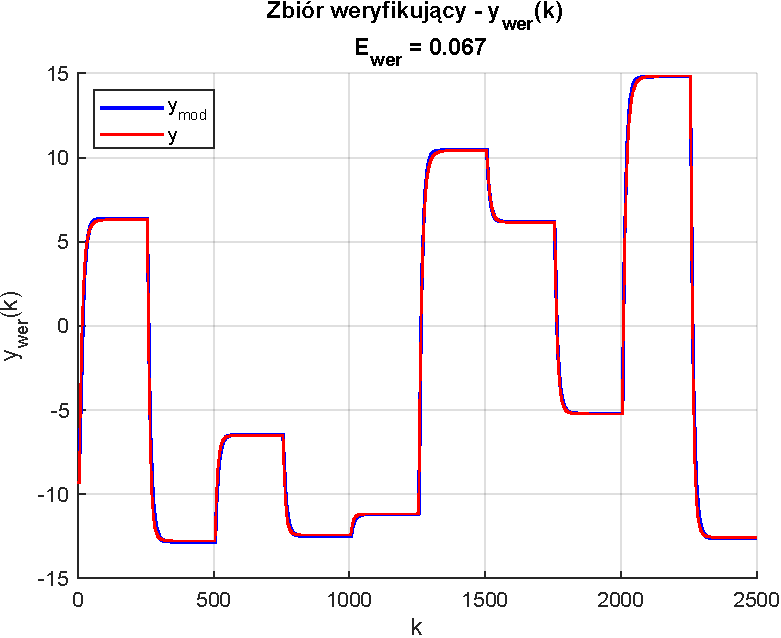
\includegraphics[width=0.45\textwidth]{pictures/oe_hamm_wer_1}}
\caption{Porównanie przebiegu sygnału wyjściowego modelu dynamicznego i modelu Hammesteina w trybie z rekurencją.}
\end{figure}

%%%%%%%%%%%%%%%%%%%%%% DRUGA SEKWENCJA %%%%%%%%%%%%%%%%%%%%%%

\begin{figure}[p!]

\begin{center}
\Large \textbf{II sekwencja} \\
\vspace{0.5cm}
\Large \textbf{Model dynamiczny}
\end{center}

\centering
\subfloat[Zbiór uczący.]{
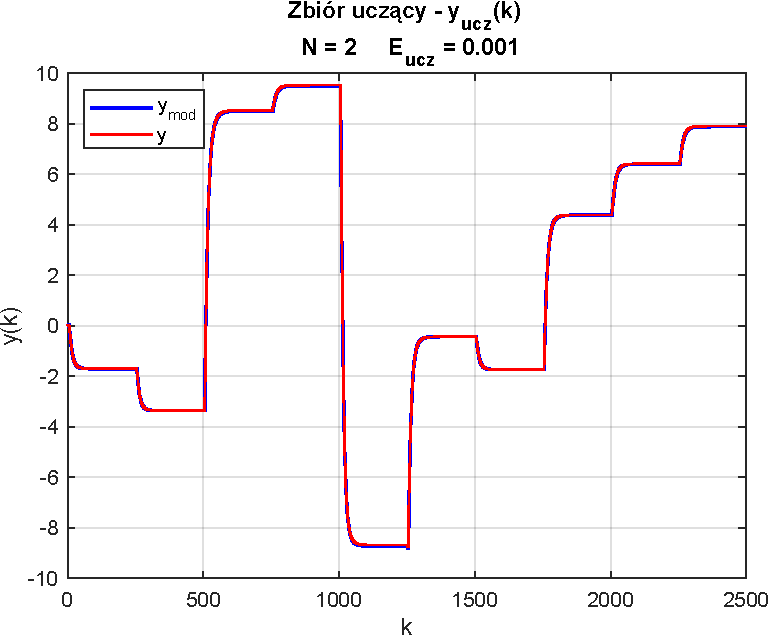
\includegraphics[width=0.45\textwidth]{pictures/arx_ucz_2}}
\hfill
\subfloat[Zbiór weryfikujący]{
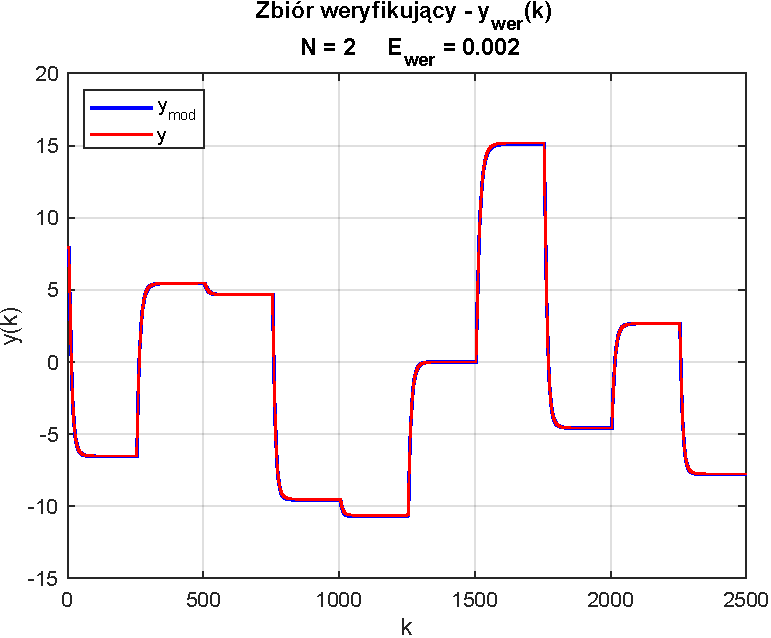
\includegraphics[width=0.45\textwidth]{pictures/arx_wer_2}}

\begin{center}
\Large \textbf{Model Hammersteina}
\end{center}

\subfloat[Zbiór uczący.]{
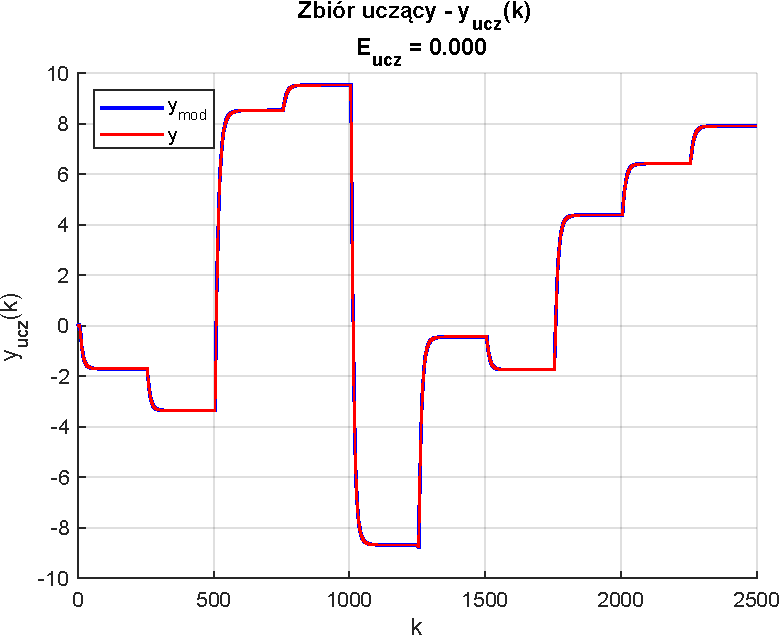
\includegraphics[width=0.45\textwidth]{pictures/arx_hamm_ucz_2}}
\hfill
\subfloat[Zbiór weryfikujący]{
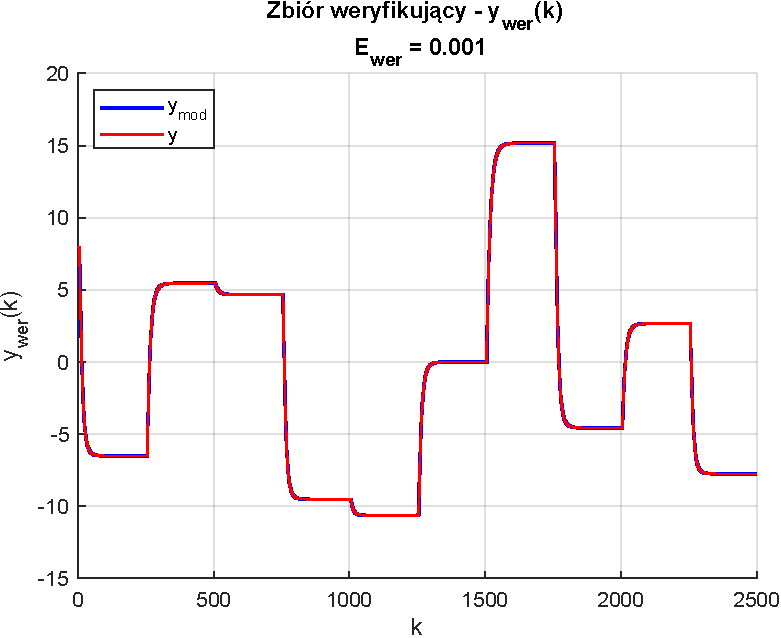
\includegraphics[width=0.45\textwidth]{pictures/arx_hamm_wer_2}}
\caption{Porównanie przebiegu sygnału wyjściowego modelu dynamicznego i modelu Hammesteina w trybie bez rekurencji.}
\end{figure}

\begin{figure}[p!]

\begin{center}
\Large \textbf{II sekwencja} \\
\vspace{0.5cm}
\Large \textbf{Model dynamiczny}
\end{center}

\centering
\subfloat[Zbiór uczący.]{
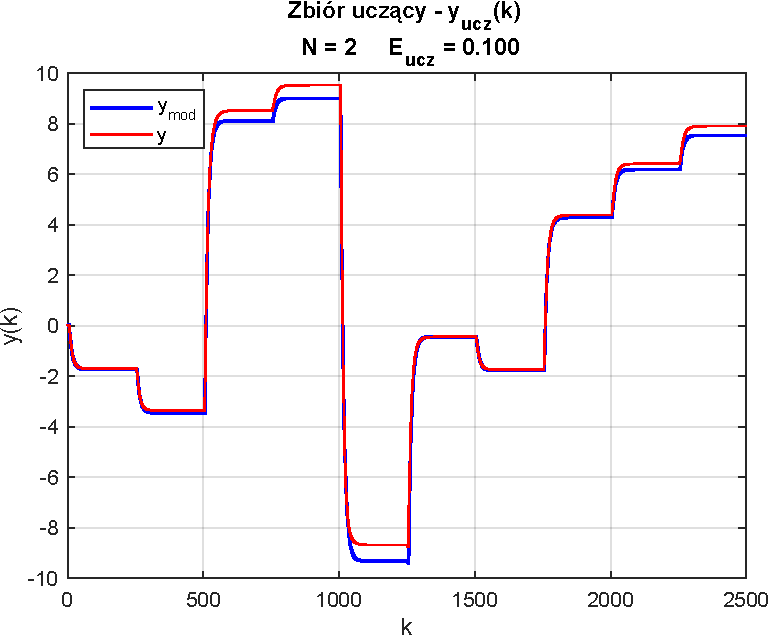
\includegraphics[width=0.45\textwidth]{pictures/oe_ucz_2}}
\hfill
\subfloat[Zbiór weryfikujący]{
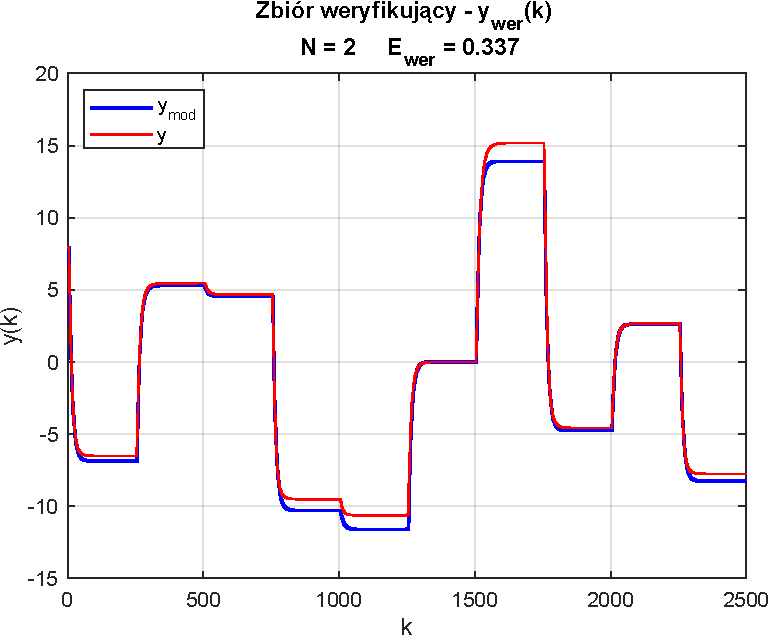
\includegraphics[width=0.45\textwidth]{pictures/oe_wer_2}}

\begin{center}
\Large \textbf{Model Hammersteina}
\end{center}

\subfloat[Zbiór uczący.]{
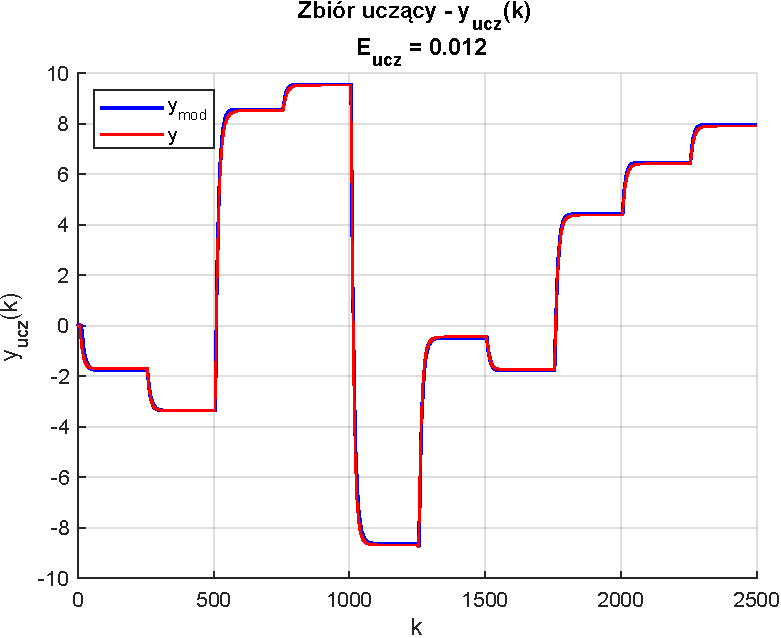
\includegraphics[width=0.45\textwidth]{pictures/oe_hamm_ucz_2}}
\hfill
\subfloat[Zbiór weryfikujący]{
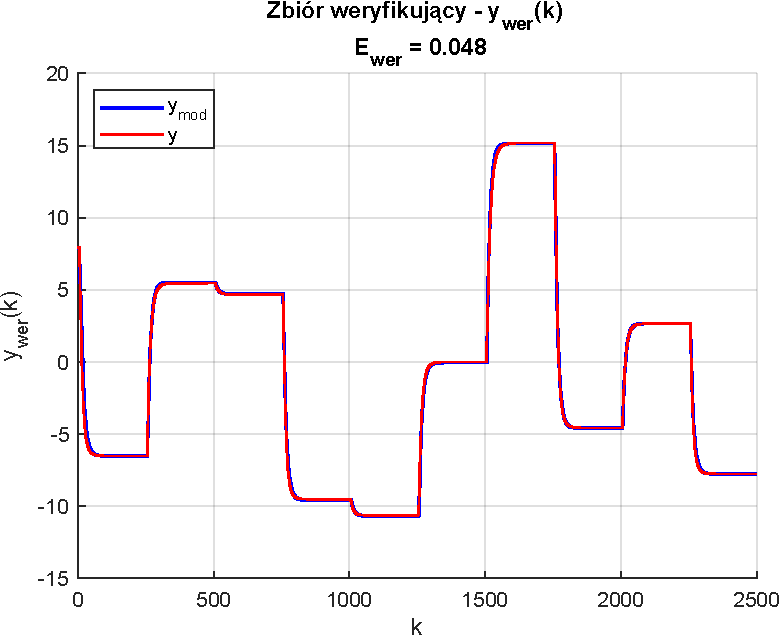
\includegraphics[width=0.45\textwidth]{pictures/oe_hamm_wer_2}}
\caption{Porównanie przebiegu sygnału wyjściowego modelu dynamicznego i modelu Hammesteina w trybie z rekurencją.}
\end{figure}

%%%%%%%%%%%%%%%%%%%%%% TRZECIA SEKWENCJA %%%%%%%%%%%%%%%%%%%%%%

\begin{figure}[p!]

\begin{center}
\Large \textbf{III sekwencja} \\
\vspace{0.5cm}
\Large \textbf{Model dynamiczny}
\end{center}

\centering
\subfloat[Zbiór uczący.]{
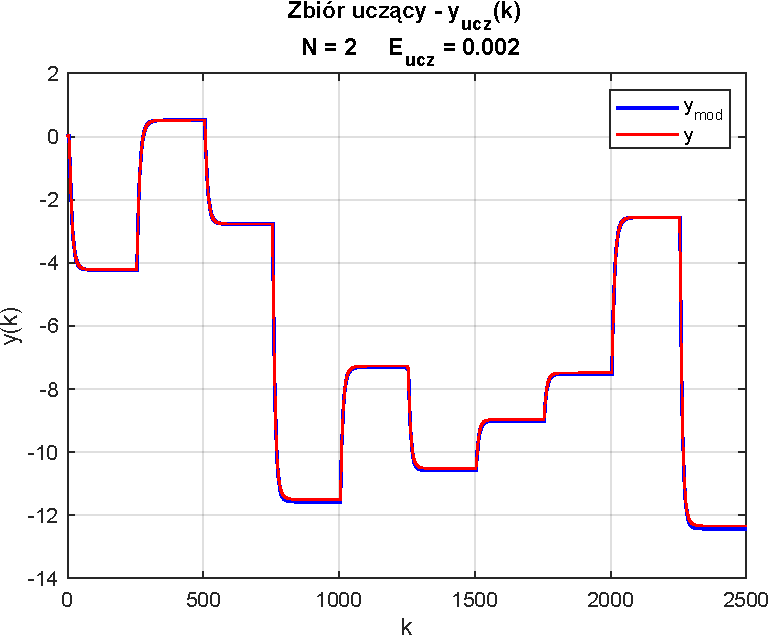
\includegraphics[width=0.45\textwidth]{pictures/arx_ucz_3}}
\hfill
\subfloat[Zbiór weryfikujący]{
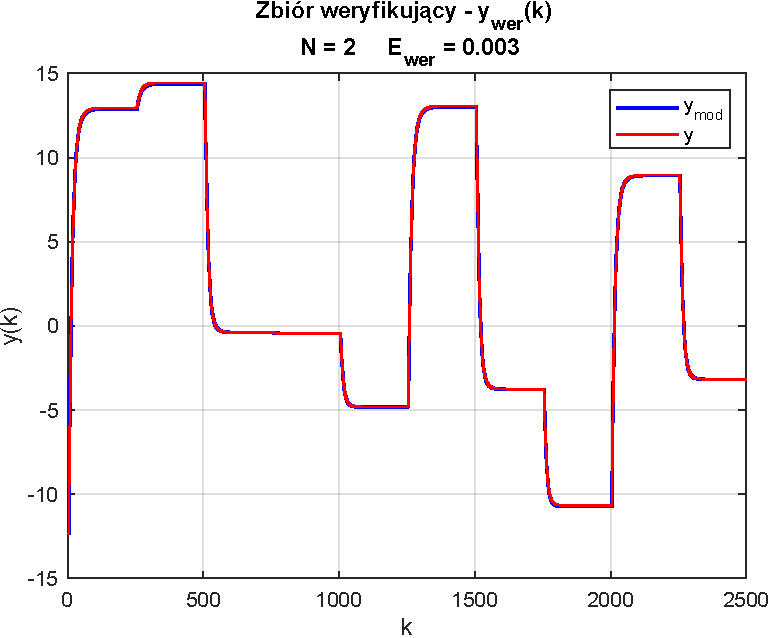
\includegraphics[width=0.45\textwidth]{pictures/arx_wer_3}}

\begin{center}
\Large \textbf{Model Hammersteina}
\end{center}

\subfloat[Zbiór uczący.]{
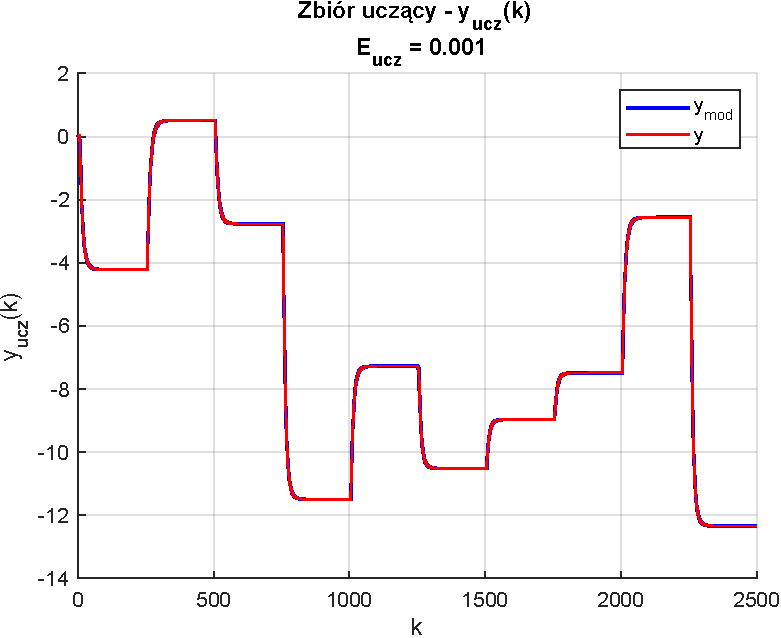
\includegraphics[width=0.45\textwidth]{pictures/arx_hamm_ucz_3}}
\hfill
\subfloat[Zbiór weryfikujący]{
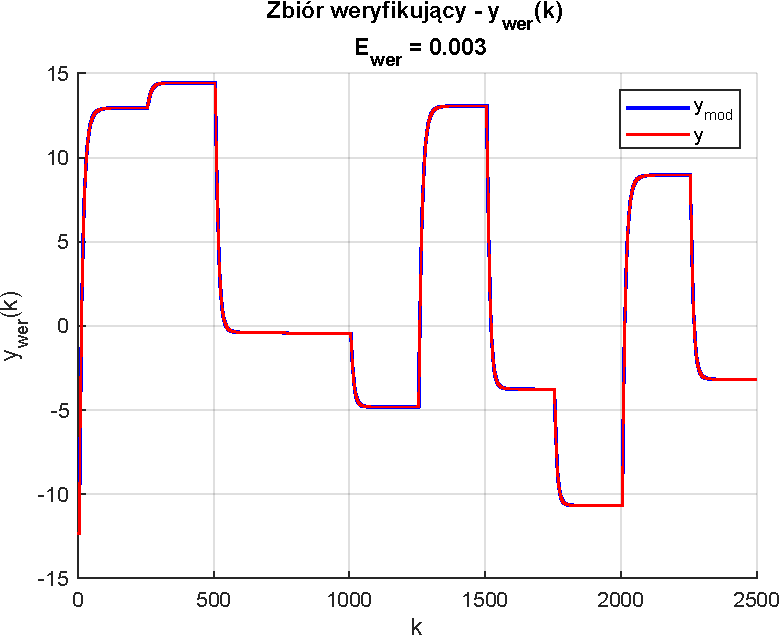
\includegraphics[width=0.45\textwidth]{pictures/arx_hamm_wer_3}}
\caption{Porównanie przebiegu sygnału wyjściowego modelu dynamicznego i modelu Hammesteina w trybie bez rekurencji.}
\end{figure}

\newpage

\begin{figure}[h!]

\begin{center}
\Large \textbf{III sekwencja} \\
\vspace{0.5cm}
\Large \textbf{Model dynamiczny}
\end{center}

\centering
\subfloat[Zbiór uczący.]{
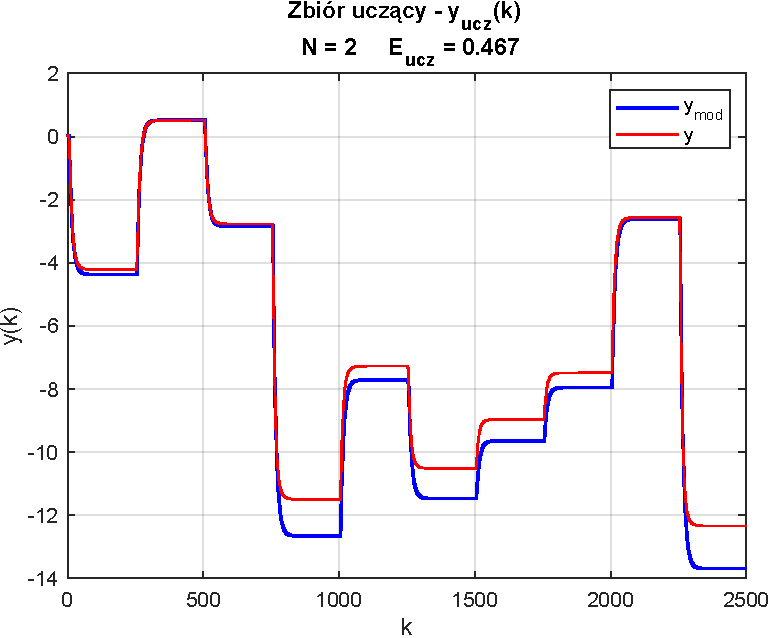
\includegraphics[width=0.45\textwidth]{pictures/oe_ucz_3}}
\hfill
\subfloat[Zbiór weryfikujący]{
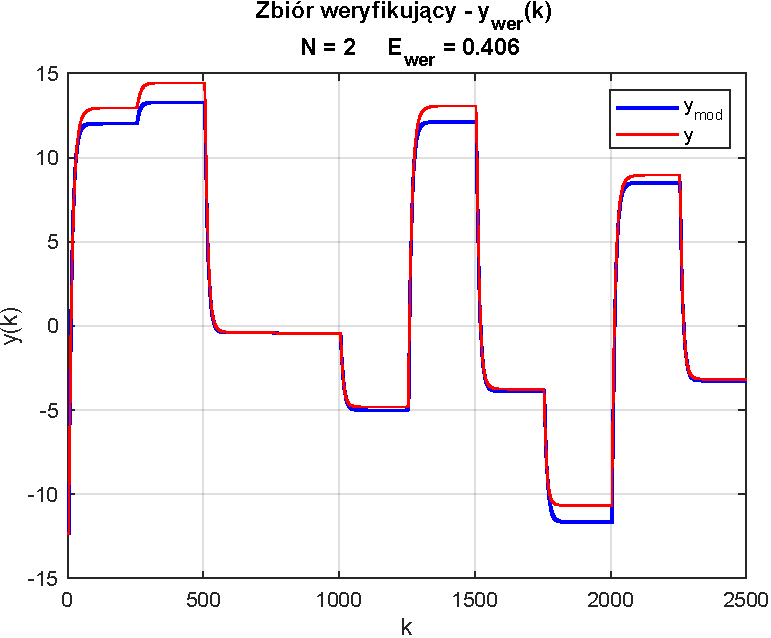
\includegraphics[width=0.45\textwidth]{pictures/oe_wer_3}}

\begin{center}
\Large \textbf{Model Hammersteina}
\end{center}

\subfloat[Zbiór uczący.]{
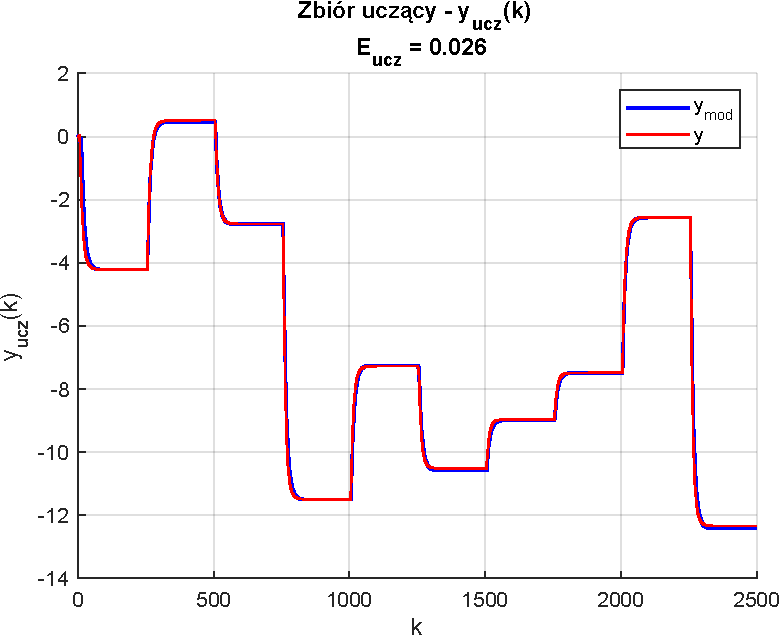
\includegraphics[width=0.45\textwidth]{pictures/oe_hamm_ucz_3}}
\hfill
\subfloat[Zbiór weryfikujący]{
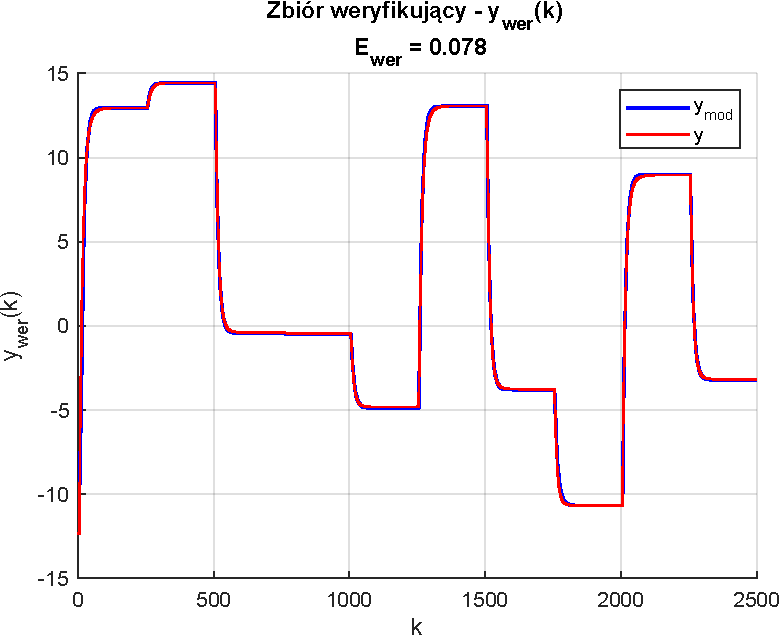
\includegraphics[width=0.45\textwidth]{pictures/oe_hamm_wer_3}}
\caption{Porównanie przebiegu sygnału wyjściowego modelu dynamicznego i modelu Hammesteina w trybie z rekurencją.}
\end{figure}

W każdym z otrzymanych przypadków model Hammersteina z rozmytą statyką i następnikami liniowymi okazywał się być lepszy niż standardowy model dynamiczny, zarówno ten testowany w trybie bez rekurencji, jak i z rekurencją. Istotnie, wprowadzenie nieliniowości do obiektu nieliniowego opisanego liniowym modelem dynamicznym poprawia dokładność otrzymywanych wyników. Jako akceptowalną granicę przyjęto błąd na poziomie $E = \num{0.1}$, a kluczowym przypadkiem był model testowany w trybie rekurencyjnym dla zbioru weryfikującego. Model Hammersteina w tej konfiguracji dawał na tyle satysfakcjonujące wyniki, że postanowiono dalej nie ingerować w dostrajanie współczynników modelu. 

\newpage

\section{Następniki hiperboliczne}
Wprowadzając dodatkową nieliniowość w opisie obiektu - poprzez zastosowanie następników hiperbolicznych - spodziewano się poprawy dokładności otrzymywanych wyników. Ponadto, zdecydowano się zmniejszyć liczbę funkcji przynależności, zachowując wcześniej uzyskaną dokładność. Wspomniane funkcje przynależności przedstawiono na rys. \ref{sets_ham_nlin}.

\begin{figure}[h!]
\centering
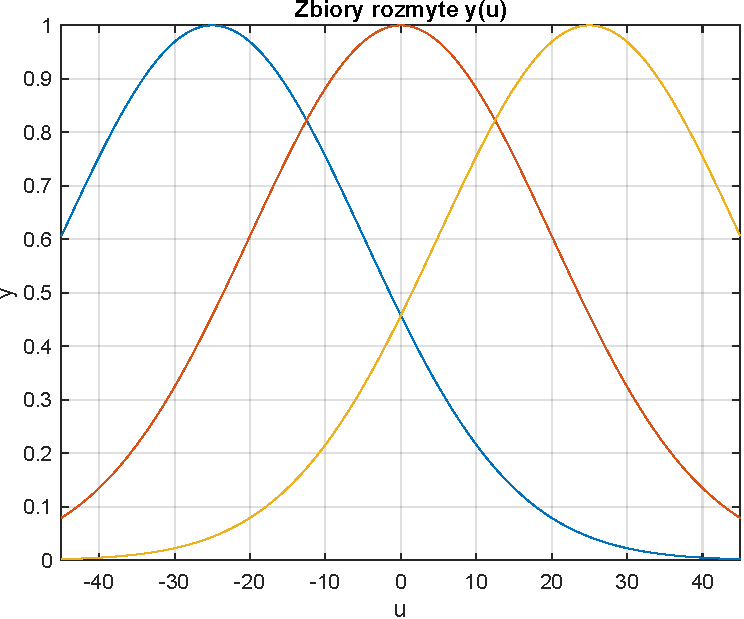
\includegraphics[width=0.5\textwidth]{pictures/fuzzy_set_ham_nlin}
\caption{Zbiory rozmyte - następniki hiperboliczne.}
\label{sets_ham_nlin}
\end{figure}

Dużo czasu poświęcono podczas dobory odpowiednich następnikom hiperbolicznych. Rozpatrzono następujące przykłady:

\begin{equation}
\begin{aligned}
y(k) &= a + \tanh(b u(k)) \\
y(k) &= a \cdot \tanh(b u(k) + c) \\
y(k) &= a + \sinh(b u(k)) \\
y(k) &= a \cdot \sinh(b u(k) + c) \\
\end{aligned} 
\end{equation}

Ostatecznie wybór padł na ostatni z przypadków - następnik wykorzystujący funkcję sinusa hiperbolicznego (rys. \ref{sinh}). 

\begin{figure}[h!]
\centering
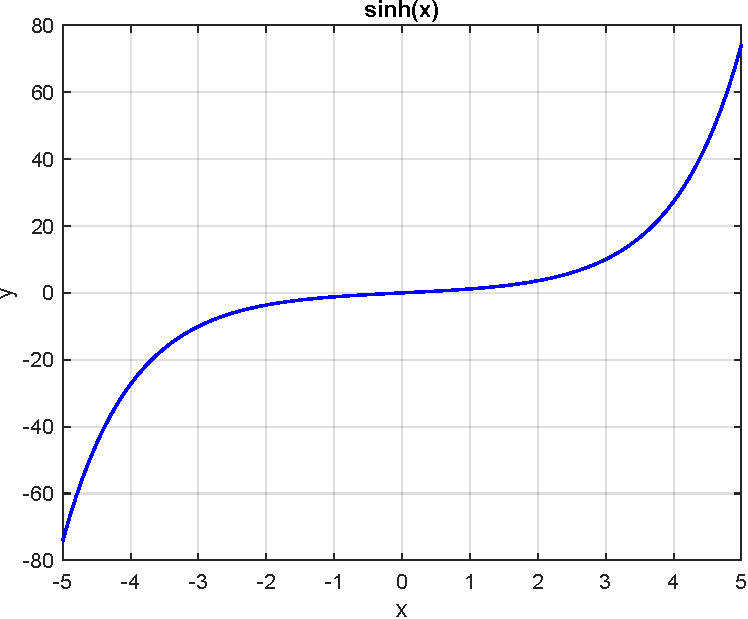
\includegraphics[width=0.5\textwidth]{pictures/sinh}
\caption{Wykres sinusa hiperbolicznego $\sinh(x)$.}
\label{sinh}
\end{figure}

\newpage

Zatem po wyborze postaci następników reguły prezentowały się następująco:

\begin{equation}
\begin{aligned}
\text{Reguła 1: Jeśli} \quad u^1(k) \quad \text{jest} \quad &U_1, \quad \text{to}: \quad y^1(k) = a_1 \cdot \sinh(b_1 u^1(k) + c_1) \\
\text{Reguła 2: Jeśli} \quad u^2(k) \quad \text{jest} \quad &U_2, \quad \text{to}: \quad y^2(k) = a_2 \cdot \sinh(b_2 u^2(k) + c_2) \\ 
\text{Reguła 3: Jeśli} \quad u^3(k) \quad \text{jest} \quad &U_3, \quad \text{to}: \quad y^3(k) = a_3 \cdot \sinh(b_3 u^3(k) + c_3) \\
\end{aligned}
\end{equation}

Po wyborze postaci następników i ilości zbiorów rozmytych rozpoczęto analizę stworzonego modelu rozmytego. Poniżej przedstawiono aproksymację charakterystyki statycznej.

\begin{figure}[h!]
\subfloat[Zbiór uczący.]{
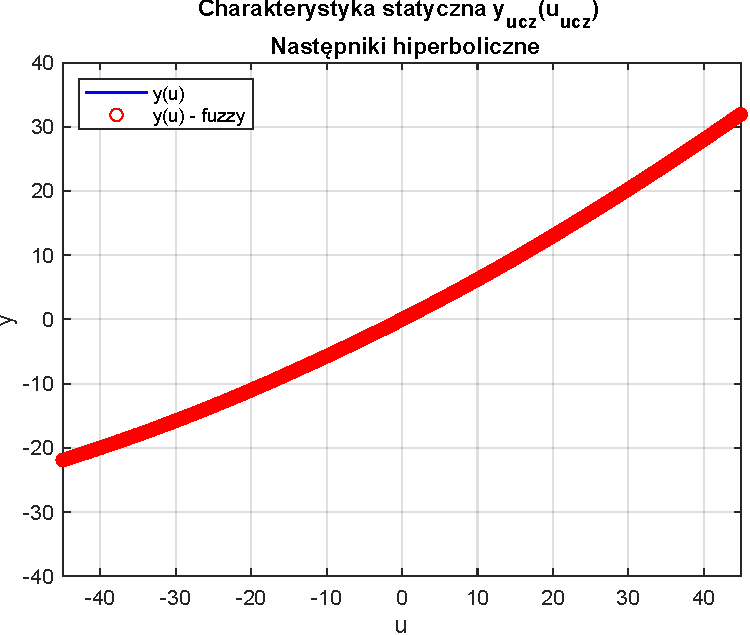
\includegraphics[width=0.45\textwidth]{pictures/static_char_ham_nlin_ucz}}
\hfill
\subfloat[Zbiór weryfikujący]{
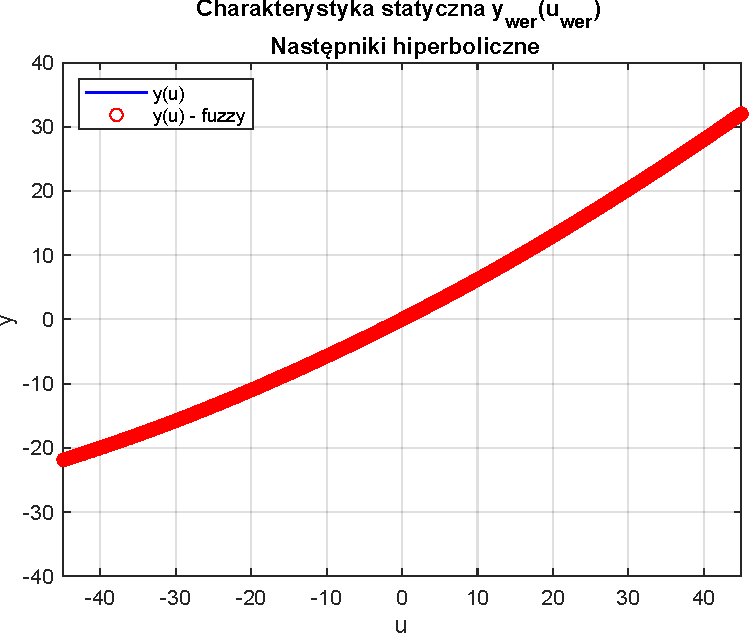
\includegraphics[width=0.45\textwidth]{pictures/static_char_ham_nlin_wer}}
\caption{Aproksymacja charakterystyki statycznej przez model rozmyty - następniki hiperboliczne.}
\end{figure}

Dokładność jest bardzo dobra, a błąd uczenia rzędu $E = \num{0.0001}$. Następnym krokiem było zbadanie zachowania modelu dla danych dynamicznych testowanych w dwóch trybach - ARX oraz OE.

%%%%%%%%%%%%%%%%%%%%%% PIERWSZA SEKWENCJA %%%%%%%%%%%%%%%%%%%%%%

\begin{figure}[p!]

\begin{center}
\Large \textbf{I sekwencja} \\
\vspace{0.5cm}
\Large \textbf{Model dynamiczny}
\end{center}

\centering
\subfloat[Zbiór uczący.]{
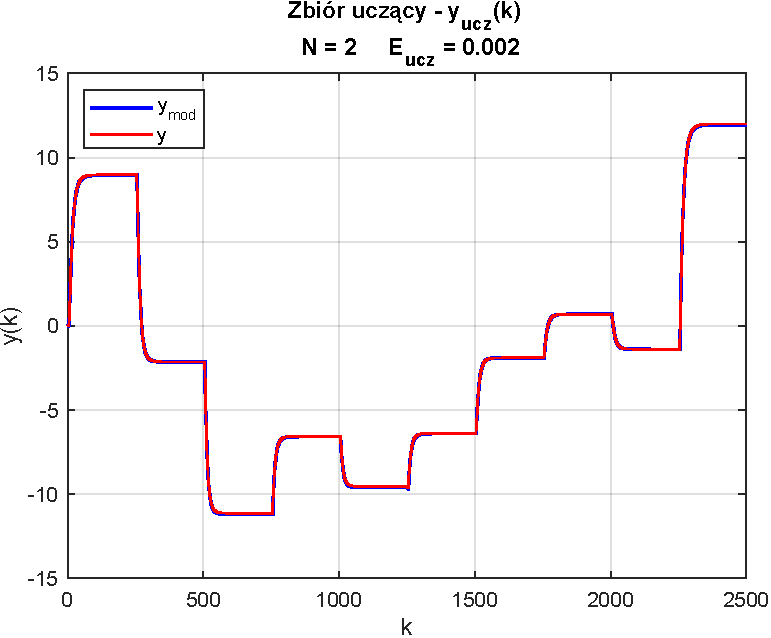
\includegraphics[width=0.45\textwidth]{pictures/arx_ucz_4}}
\hfill
\subfloat[Zbiór weryfikujący]{
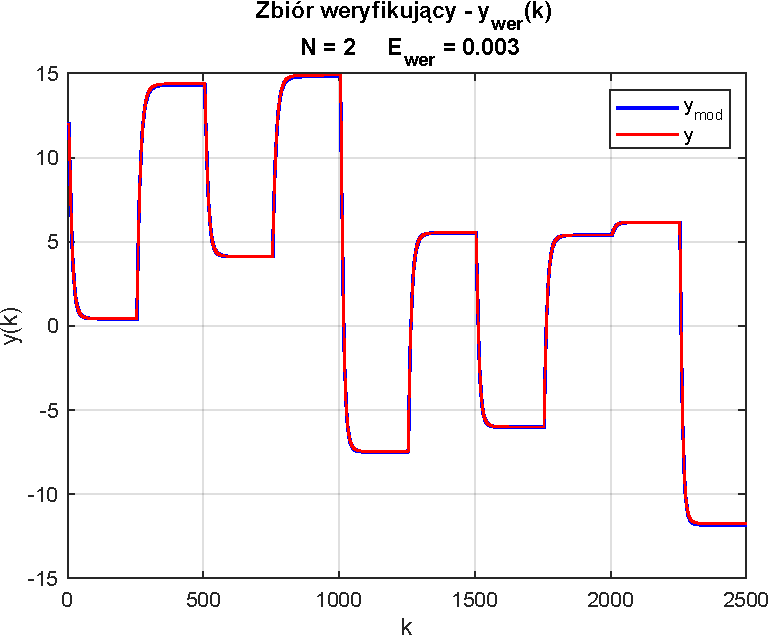
\includegraphics[width=0.45\textwidth]{pictures/arx_wer_4}}

\begin{center}
\Large \textbf{Model Hammersteina}
\end{center}

\subfloat[Zbiór uczący.]{
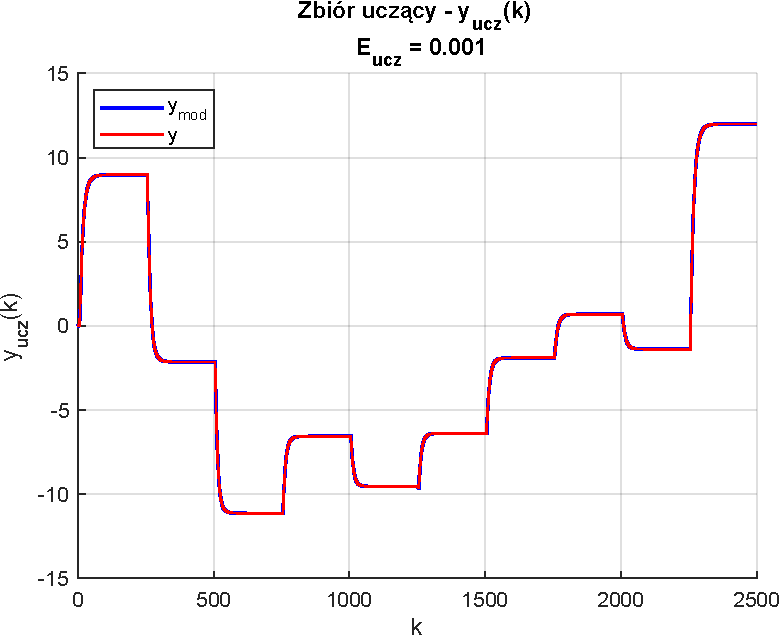
\includegraphics[width=0.45\textwidth]{pictures/arx_hamm_ucz_4}}
\hfill
\subfloat[Zbiór weryfikujący]{
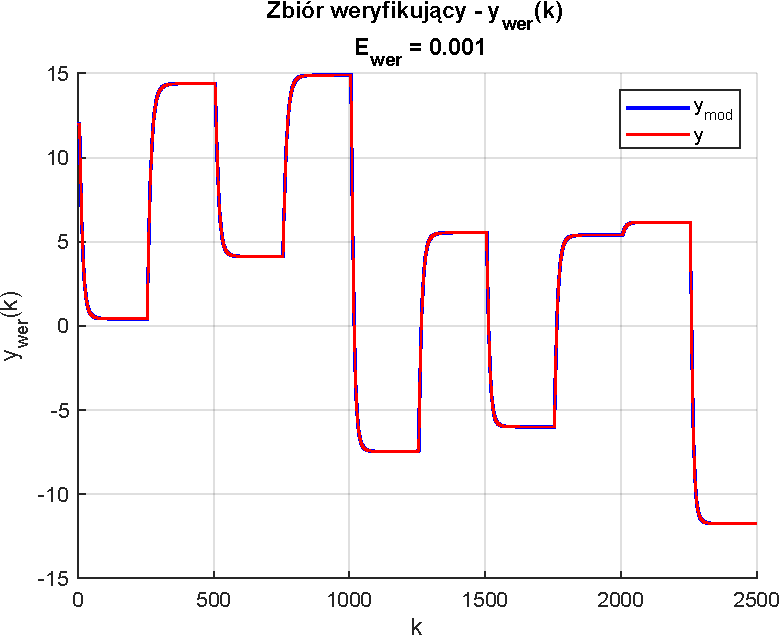
\includegraphics[width=0.45\textwidth]{pictures/arx_hamm_wer_4}}
\caption{Porównanie przebiegu sygnału wyjściowego modelu dynamicznego i modelu Hammesteina w trybie bez rekurencji.}
\end{figure} 
 
\begin{figure}[p!]

\begin{center}
\Large \textbf{I sekwencja} \\
\vspace{0.5cm}
\Large \textbf{Model dynamiczny}
\end{center}

\centering
\subfloat[Zbiór uczący.]{
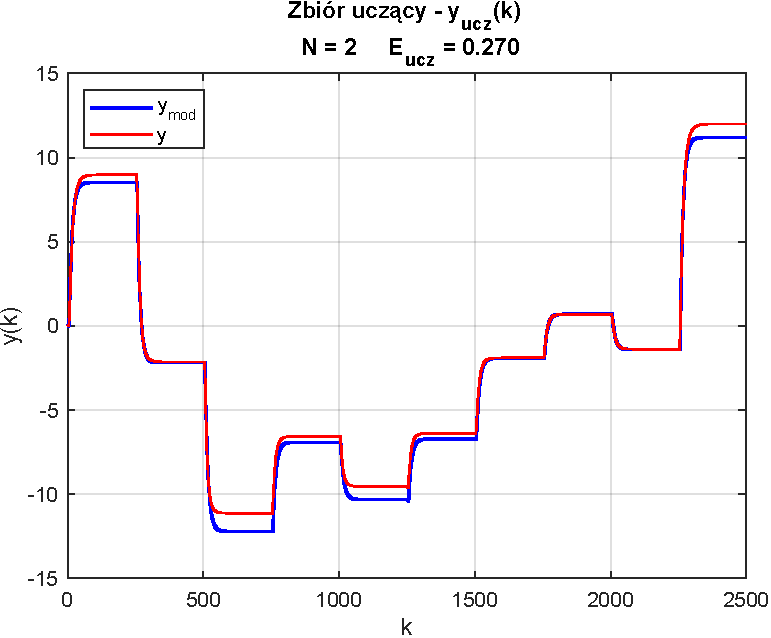
\includegraphics[width=0.45\textwidth]{pictures/oe_ucz_4}}
\hfill
\subfloat[Zbiór weryfikujący]{
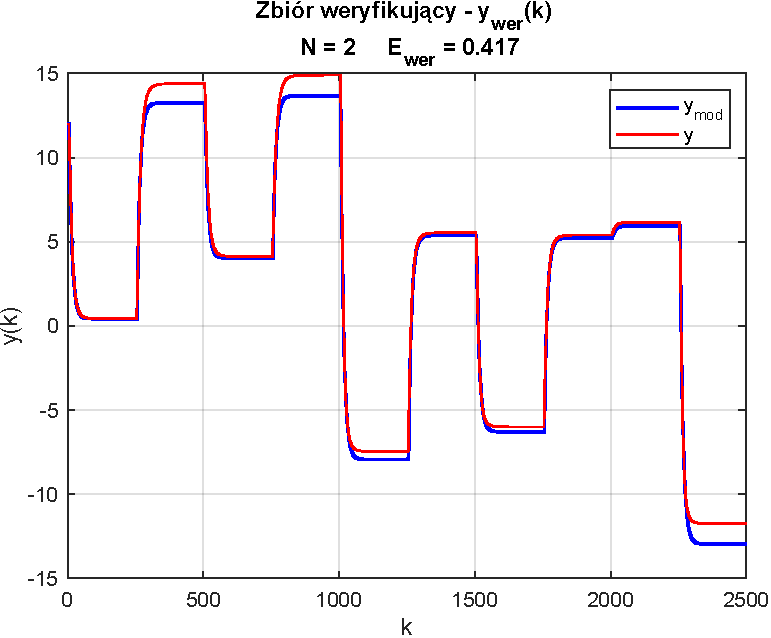
\includegraphics[width=0.45\textwidth]{pictures/oe_wer_4}}

\begin{center}
\Large \textbf{Model Hammersteina}
\end{center}

\subfloat[Zbiór uczący.]{
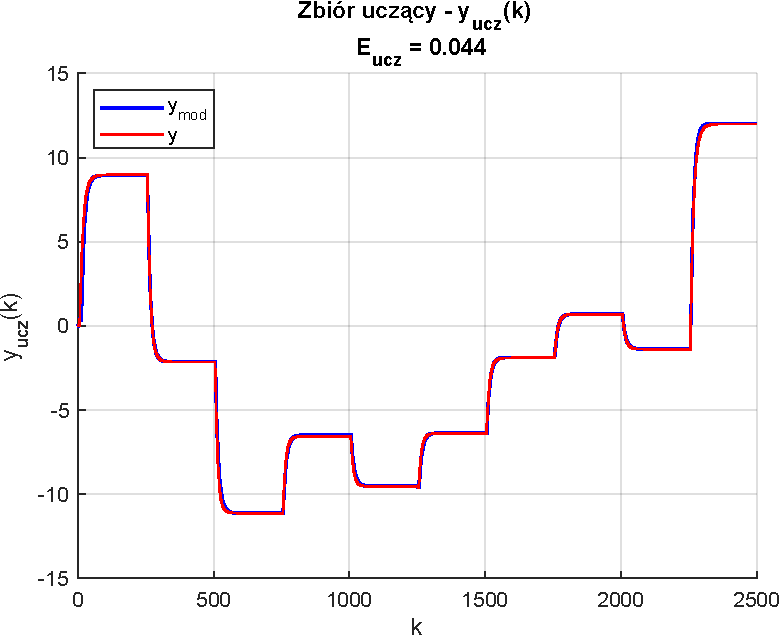
\includegraphics[width=0.45\textwidth]{pictures/oe_hamm_ucz_4}}
\hfill
\subfloat[Zbiór weryfikujący]{
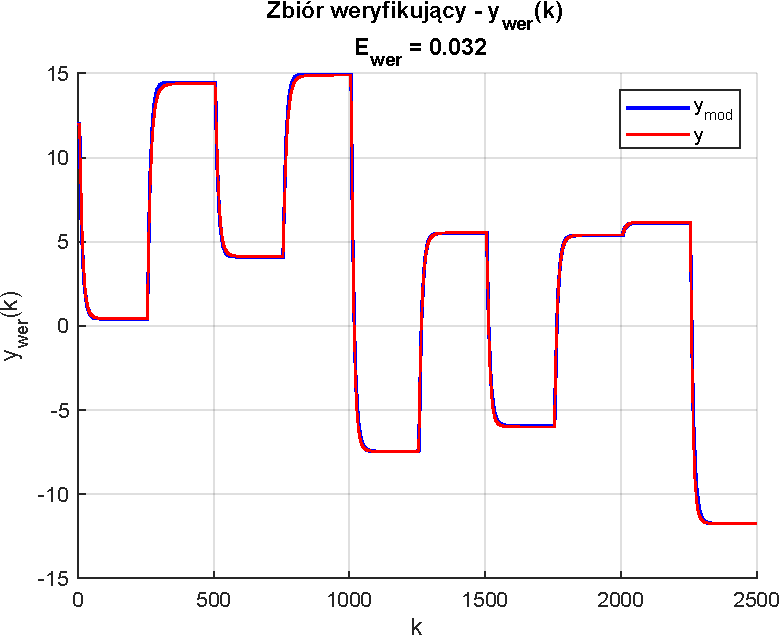
\includegraphics[width=0.45\textwidth]{pictures/oe_hamm_wer_4}}
\caption{Porównanie przebiegu sygnału wyjściowego modelu dynamicznego i modelu Hammesteina w trybie z rekurencją.}
\end{figure} 

%%%%%%%%%%%%%%%%%%%%%% DRUGA SEKWENCJA %%%%%%%%%%%%%%%%%%%%%%
\begin{figure}[p!]

\begin{center}
\Large \textbf{II sekwencja} \\
\vspace{0.5cm}
\Large \textbf{Model dynamiczny}
\end{center}

\centering
\subfloat[Zbiór uczący.]{
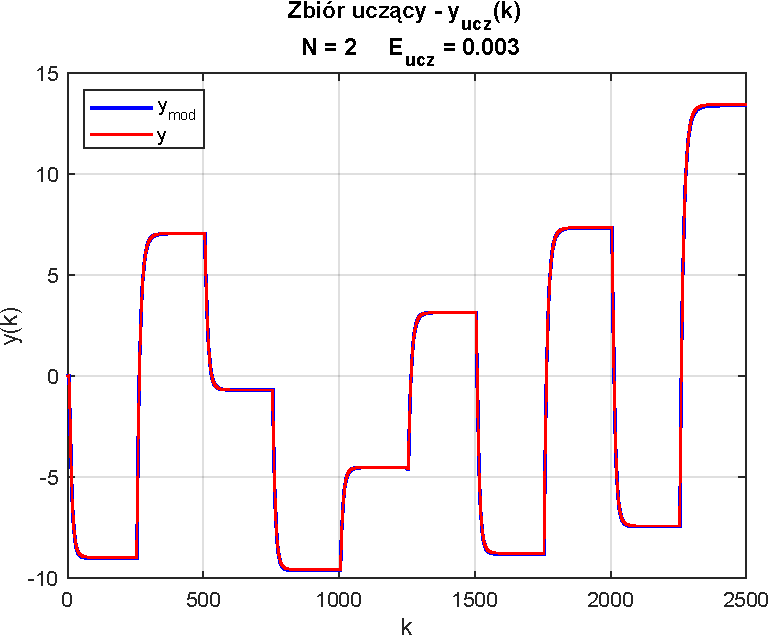
\includegraphics[width=0.45\textwidth]{pictures/arx_ucz_5}}
\hfill
\subfloat[Zbiór weryfikujący]{
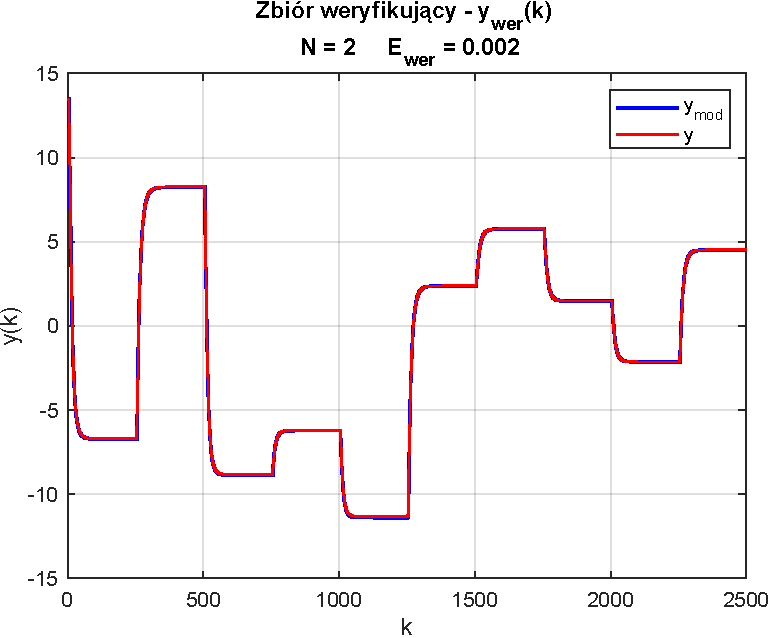
\includegraphics[width=0.45\textwidth]{pictures/arx_wer_5}}

\begin{center}
\Large \textbf{Model Hammersteina}
\end{center}

\subfloat[Zbiór uczący.]{
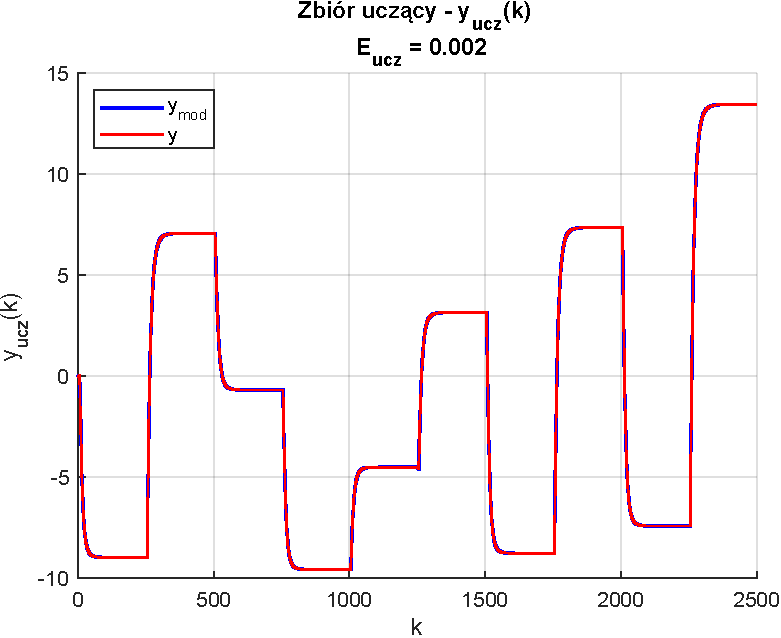
\includegraphics[width=0.45\textwidth]{pictures/arx_hamm_ucz_5}}
\hfill
\subfloat[Zbiór weryfikujący]{
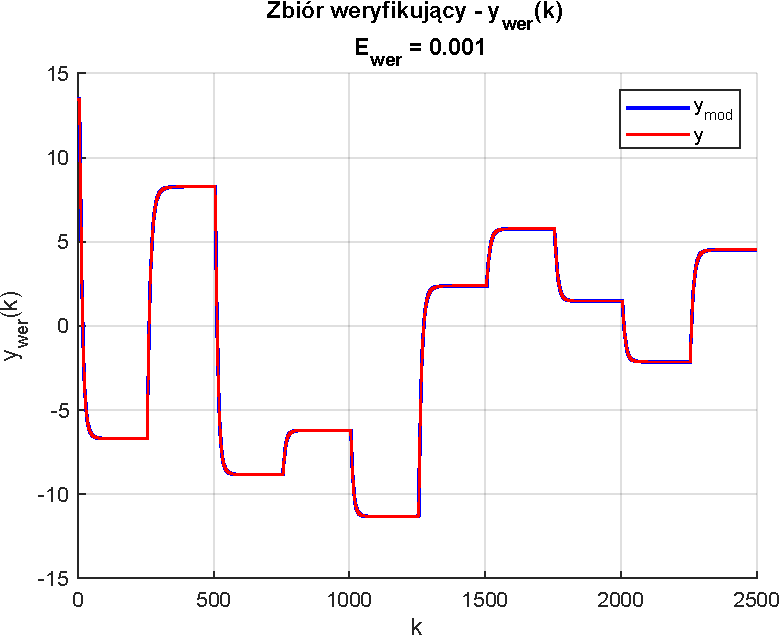
\includegraphics[width=0.45\textwidth]{pictures/arx_hamm_wer_5}}
\caption{Porównanie przebiegu sygnału wyjściowego modelu dynamicznego i modelu Hammesteina w trybie bez rekurencji.}
\end{figure} 
 
\begin{figure}[p!]

\begin{center}
\Large \textbf{II sekwencja} \\
\vspace{0.5cm}
\Large \textbf{Model dynamiczny}
\end{center}

\centering
\subfloat[Zbiór uczący.]{
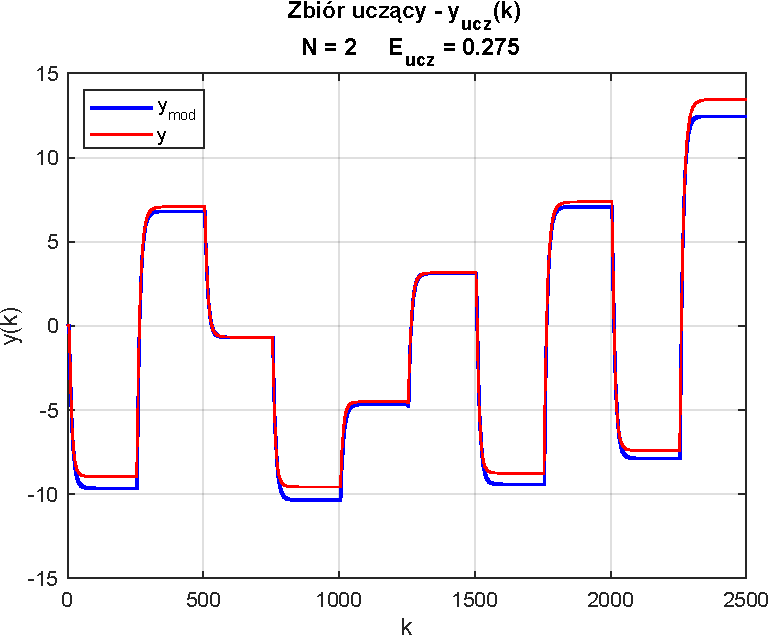
\includegraphics[width=0.45\textwidth]{pictures/oe_ucz_5}}
\hfill
\subfloat[Zbiór weryfikujący]{
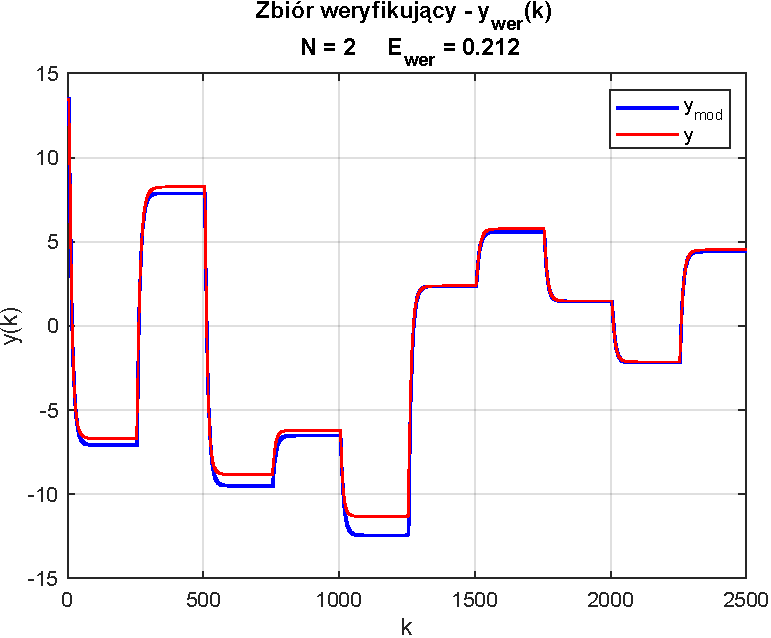
\includegraphics[width=0.45\textwidth]{pictures/oe_wer_5}}

\begin{center}
\Large \textbf{Model Hammersteina}
\end{center}

\subfloat[Zbiór uczący.]{
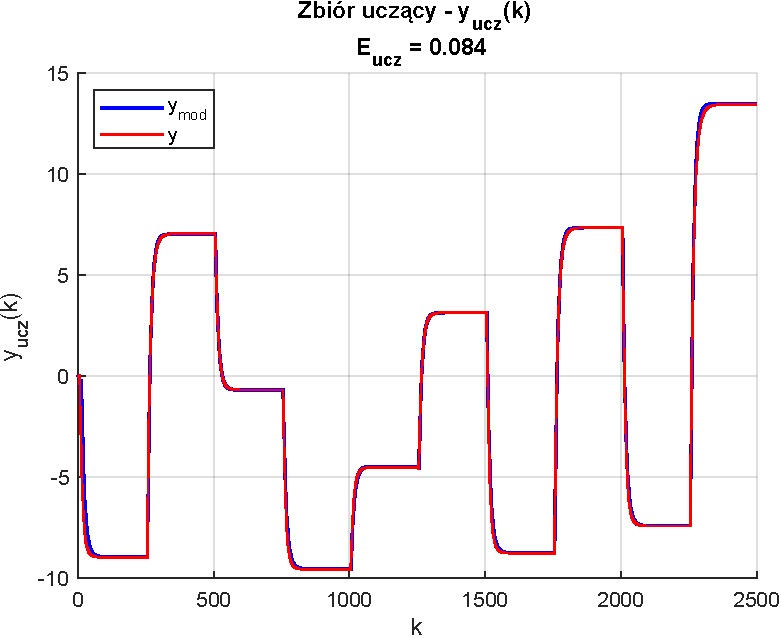
\includegraphics[width=0.45\textwidth]{pictures/oe_hamm_ucz_5}}
\hfill
\subfloat[Zbiór weryfikujący]{
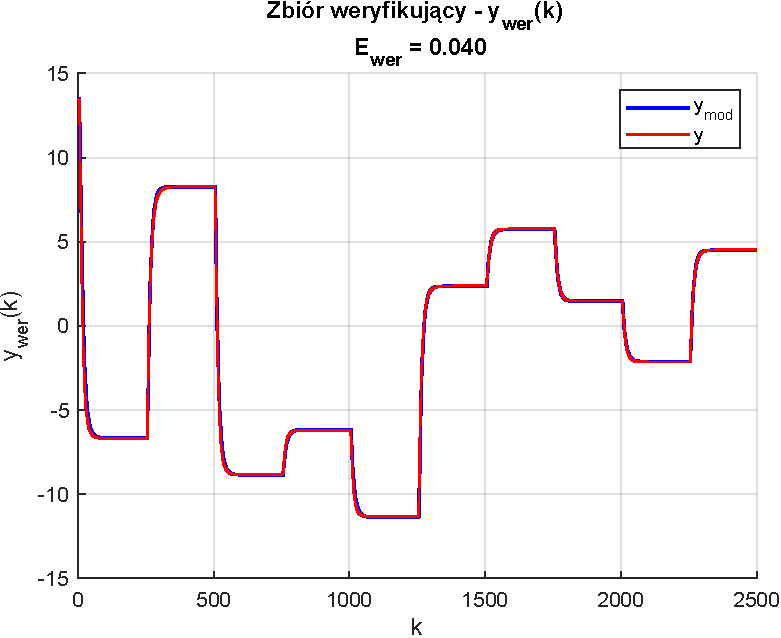
\includegraphics[width=0.45\textwidth]{pictures/oe_hamm_wer_5}}
\caption{Porównanie przebiegu sygnału wyjściowego modelu dynamicznego i modelu Hammesteina w trybie z rekurencją.}
\end{figure} 

%%%%%%%%%%%%%%%%%%%%%% TRZECIA SEKWENCJA %%%%%%%%%%%%%%%%%%%%%%
\begin{figure}[p!]

\begin{center}
\Large \textbf{III sekwencja} \\
\vspace{0.5cm}
\Large \textbf{Model dynamiczny}
\end{center}

\centering
\subfloat[Zbiór uczący.]{
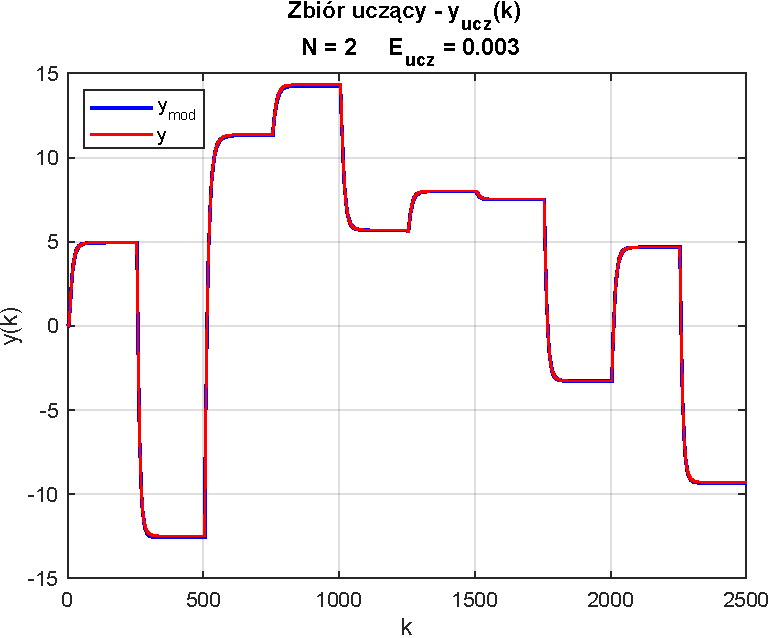
\includegraphics[width=0.45\textwidth]{pictures/arx_ucz_6}}
\hfill
\subfloat[Zbiór weryfikujący]{
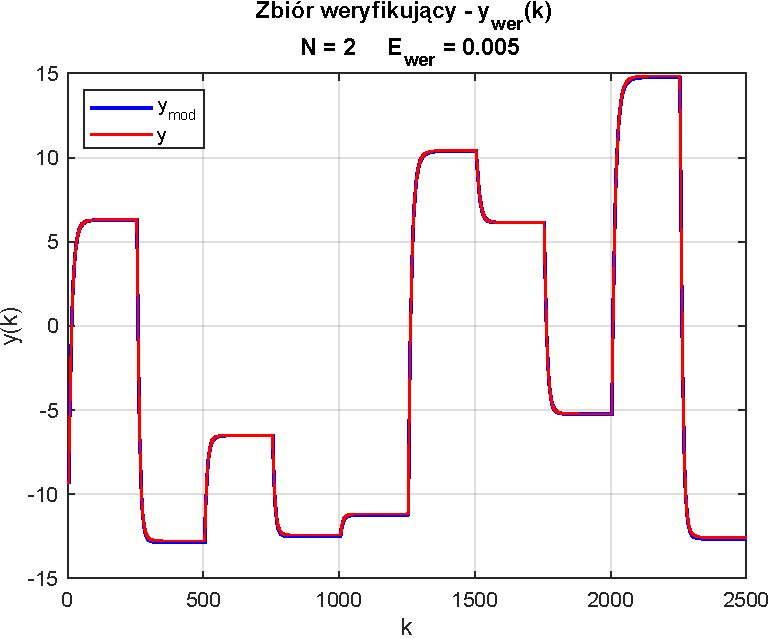
\includegraphics[width=0.45\textwidth]{pictures/arx_wer_6}}

\begin{center}
\Large \textbf{Model Hammersteina}
\end{center}

\subfloat[Zbiór uczący.]{
\includegraphics[width=0.45\textwidth]{pictures/arx_hamm_ucz_6}}
\hfill
\subfloat[Zbiór weryfikujący]{
\includegraphics[width=0.45\textwidth]{pictures/arx_hamm_wer_6}}
\caption{Porównanie przebiegu sygnału wyjściowego modelu dynamicznego i modelu Hammesteina w trybie bez rekurencji.}
\end{figure} 

\newpage
 
\begin{figure}[h!]

\begin{center}
\Large \textbf{III sekwencja} \\
\vspace{0.5cm}
\Large \textbf{Model dynamiczny}
\end{center}

\centering
\subfloat[Zbiór uczący.]{
\includegraphics[width=0.45\textwidth]{pictures/oe_ucz_6}}
\hfill
\subfloat[Zbiór weryfikujący]{
\includegraphics[width=0.45\textwidth]{pictures/oe_wer_6}}

\begin{center}
\Large \textbf{Model Hammersteina}
\end{center}

\subfloat[Zbiór uczący.]{
\includegraphics[width=0.45\textwidth]{pictures/oe_hamm_ucz_6}}
\hfill
\subfloat[Zbiór weryfikujący]{
\includegraphics[width=0.45\textwidth]{pictures/oe_hamm_wer_6}}
\caption{Porównanie przebiegu sygnału wyjściowego modelu dynamicznego i modelu Hammesteina w trybie z rekurencją.}
\end{figure} 

Na podstawie powyższych wykresów można wysnuć wniosek, że cel został osiągnięty. Przy mniejszej liczbie zbiorów rozmytych udało się uzyskać tą samą dokładność, jak w przypadku następników liniowych. Ponownie, jakość opisu obiektu uznano na tyle dobry, że postanowiono nie stroić modelu ręcznie. Reasumując, wprowadzenie dodatkowej nieliniowości w postaci następników hiperbolicznych pozwala osiągnąć satysfakcjonujące rezultaty.